% Options for packages loaded elsewhere
\PassOptionsToPackage{unicode}{hyperref}
\PassOptionsToPackage{hyphens}{url}
\documentclass[
  11pt,
]{article}
\usepackage{xcolor}
\usepackage[margin=1in]{geometry}
\usepackage{amsmath,amssymb}
\setcounter{secnumdepth}{-\maxdimen} % remove section numbering
\usepackage{iftex}
\ifPDFTeX
  \usepackage[T1]{fontenc}
  \usepackage[utf8]{inputenc}
  \usepackage{textcomp} % provide euro and other symbols
\else % if luatex or xetex
  \usepackage{unicode-math} % this also loads fontspec
  \defaultfontfeatures{Scale=MatchLowercase}
  \defaultfontfeatures[\rmfamily]{Ligatures=TeX,Scale=1}
\fi
\usepackage{lmodern}
\ifPDFTeX\else
  % xetex/luatex font selection
\fi
% Use upquote if available, for straight quotes in verbatim environments
\IfFileExists{upquote.sty}{\usepackage{upquote}}{}
\IfFileExists{microtype.sty}{% use microtype if available
  \usepackage[]{microtype}
  \UseMicrotypeSet[protrusion]{basicmath} % disable protrusion for tt fonts
}{}
\makeatletter
\@ifundefined{KOMAClassName}{% if non-KOMA class
  \IfFileExists{parskip.sty}{%
    \usepackage{parskip}
  }{% else
    \setlength{\parindent}{0pt}
    \setlength{\parskip}{6pt plus 2pt minus 1pt}}
}{% if KOMA class
  \KOMAoptions{parskip=half}}
\makeatother
\usepackage{longtable,booktabs,array}
\newcounter{none} % for unnumbered tables
\usepackage{calc} % for calculating minipage widths
% Correct order of tables after \paragraph or \subparagraph
\usepackage{etoolbox}
\makeatletter
\patchcmd\longtable{\par}{\if@noskipsec\mbox{}\fi\par}{}{}
\makeatother
% Allow footnotes in longtable head/foot
\IfFileExists{footnotehyper.sty}{\usepackage{footnotehyper}}{\usepackage{footnote}}
\makesavenoteenv{longtable}
\usepackage{graphicx}
\makeatletter
\newsavebox\pandoc@box
\newcommand*\pandocbounded[1]{% scales image to fit in text height/width
  \sbox\pandoc@box{#1}%
  \Gscale@div\@tempa{\textheight}{\dimexpr\ht\pandoc@box+\dp\pandoc@box\relax}%
  \Gscale@div\@tempb{\linewidth}{\wd\pandoc@box}%
  \ifdim\@tempb\p@<\@tempa\p@\let\@tempa\@tempb\fi% select the smaller of both
  \ifdim\@tempa\p@<\p@\scalebox{\@tempa}{\usebox\pandoc@box}%
  \else\usebox{\pandoc@box}%
  \fi%
}
% Set default figure placement to htbp
\def\fps@figure{htbp}
\makeatother
\setlength{\emergencystretch}{3em} % prevent overfull lines
\providecommand{\tightlist}{%
  \setlength{\itemsep}{0pt}\setlength{\parskip}{0pt}}
\usepackage[]{natbib}
\bibliographystyle{plainnat}
\usepackage{bookmark}
\IfFileExists{xurl.sty}{\usepackage{xurl}}{} % add URL line breaks if available
\urlstyle{same}
\hypersetup{
  pdftitle={Lossless in Theory{,} Divergent in Practice: Does Adaptive Speculative Decoding Actually Pay Off?},
  pdfauthor={Author details to be confirmed},
  hidelinks,
  pdfcreator={LaTeX via pandoc}}

\title{Lossless in Theory, Divergent in Practice: Does Adaptive
Speculative Decoding Actually Pay Off?}
\author{Author details to be confirmed}
\date{Working draft --- 29 September 2026}

\begin{document}
\maketitle
\begin{abstract}
Speculative decoding is usually described as lossless: verified drafts
should reproduce the target model's own output. In a preregistered
evaluation of adaptive draft-length selection on one Apple Silicon Mac
with 24 GB unified memory, that guarantee did not hold in our
implementation: all speculative arms agree with one another on tokens
and stopping outcomes, but 9 of 20 requests differ from solo decoding.
Shorter drafts can reduce local inference latency but can also discard
useful accepted work; we evaluate a frozen acceptance-history policy for
choosing draft length. A four-arm development comparison on 20 requests,
with six scored repeats per arm, measures a 4.50\% mean paired
request-relative latency reduction versus fixed block 5 (95\%
group-bootstrap interval, 0.49--8.52\%). Its 2.76\% advantage over fixed
block 3 remains uncertain (-0.70--6.26\%), and the result misses the
registered 5\% practical-gain threshold. Saved traces motivate a
separately measured full-acceptance refresh candidate. A later
comparison on the same spent requests measures 7.13\% for refresh versus
fixed5 (2.99--11.34\%) and 7.03\% for the original policy
(2.87--11.22\%); refresh's incremental 0.11\% gain remains uncertain
(-0.075--0.335\%). The predeclared selection rule therefore retains the
original policy for confirmation. The later session uses an explicitly
amended GPU residency loader; it does not isolate loading's effect on
latency. Earlier sessions and failed attempts are retained, and repeated
measurements on spent requests are not independent confirmation. A
CPU-only audit on a separate 16 GB M4 reproduced four earlier saved
statistical comparisons exactly. A separate pre-registered test of
self-distilling the drafter on the owner's own traffic against the stock
target returned INCONCLUSIVE: an acceptance-targeted objective moved
per-prompt acceptance by +1.4 points (97.5 \% interval −0.8 to +4.1)
against a registered +3.0-point bar, distillation by +0.2, with outputs
byte-identical and no change in pooled acceptance or speed.
Fresh-request confirmation, numerical-cause diagnosis and second-machine
inference replication remain open.
\end{abstract}

\section{Introduction}\label{introduction}

Local inference imposes a joint constraint on model residency,
verification work, transient memory allocations, and whatever else is
sharing the machine. Speculative decoding amortizes target-model
evaluation across several tokens by using a cheaper proposal mechanism,
then verifying the proposals in one target pass. Its effectiveness
depends on how much proposed work is accepted \emph{and} on how
expensive a complete speculative round becomes --- higher acceptance
alone does not imply lower request latency.

Our project began with a practical question: can a personal drafter
improve as it observes one user's workload? Answering it produced a
training and evaluation repository, \texttt{mlx-mtp-tuning}, and a
separate serving repository, Whetstone. Along the way the experimental
record grew to include compatibility tests, hidden-state capture,
drafter training, candidate gates, memory failures, cache restoration,
numerical-fidelity probes, serving-path profiling, and adaptive block
selection. This paper treats that record as several distinct experiments
rather than folding their numbers into one headline performance claim.

The central controlled result is a completed four-arm comparison of
fixed block 3, fixed block 5, the frozen adaptive rule, and a duplicate
fixed-block-5 control. An acceptance-history rule switches between short
and deep speculative blocks using past accepted-token counts together
with frozen development costs. Its average improvement is positive, but
neither uniform across requests nor sufficient to establish superiority
over the best static policy. The rule is implemented in Whetstone's
controller path, where the inspected version permits it only in shadow
mode pending further evaluation.

We organize the study around three questions:

\begin{enumerate}
\def\labelenumi{\arabic{enumi}.}
\tightlist
\item
  Does the frozen rule reduce latency relative to fixed block 5, under a
  specified implementation and workload?
\item
  What computation is held constant when we assert output agreement
  between arms?
\item
  How far do development measurements and a simple workload-cost model
  justify expectations about deployment?
\end{enumerate}

A fourth, negative result sets a boundary on all three: the failed
personalization experiment shows that a functioning
mine--capture--train--judge pipeline does not by itself demonstrate
useful learning.

This draft's contribution is a bounded empirical systems study with
auditable controls, a practical block-selection implementation, and
explicit limitations. We do not claim to introduce adaptive speculative
decoding or to establish a new state of the art. The proposal to predict
benefit from a workload's output-length distribution is promising but
needs broader validation before it can carry the paper's headline claim.

\section{Related work}\label{related-work}

Speculative decoding and speculative sampling established how proposals
can accelerate target generation while preserving the target
distribution under the algorithm's assumptions
\citep{leviathan2023, chen2023}. Multi-token prediction is also a
training paradigm; the presence of an MTP inference head here should not
be confused with reproducing the broader training results of Gloeckle et
al. \citep{gloeckle2024}.

Adaptive proposal length already has substantial prior art. SpecDec++
uses a trained acceptance predictor to decide when to verify
\citep{huang2025}. DISCO dynamically selects speculation lookahead and
compares against the best static lookahead \citep{mamou2024}. BanditSpec
formulates adaptive configuration selection as a bandit problem,
requiring no training \citep{hou2025}. TapOut generalizes that idea with
an online sequence-level bandit that selects a speculation-length arm
per request, explicitly targeting the failure mode of hand-tuned fixed
or entropy thresholds that do not transfer across models and domains
\citep{sridhar2025tapout}. SVIP instead uses the draft model's own
token-level predictive entropy, training-free, as a proxy for expected
acceptance and stops a draft run early when entropy spikes
\citep{zhang2024svip}. PACER adapts block length from a
verification-time signal inside the block itself, via blockwise
pre-verification, rather than from a rolling historical statistic
\citep{zhang2026pacer}. Cascade uses speculation utility and periodic
test/set phases for mixture-of-experts models \citep{saxena2025}. Our
rule is a simple two-state special case of this broader design space ---
a frozen threshold switch between two block depths driven by rolling
acceptance history and a frozen cost model, with no online learning and
no per-token confidence signal --- so choosing between two block lengths
from observed acceptance is not, by itself, a novelty claim. A
separately completed five-arm development session includes a local
TapOut cap-4 adaptation under our verifier (Section 6.4). That adapter
is not a reproduction of the paper's complete evaluation; other named
methods remain unmeasured here.

The EAGLE family targets a related but distinct axis: drafting at the
feature level and reshaping the \emph{tree} of proposals rather than
switching a scalar depth. EAGLE resolves feature-level uncertainty by
drafting from second-to-top-layer hidden states plus a one-step-advanced
token \citep{li2024eagle}; EAGLE-2 replaces a static draft tree with a
context-dependent dynamic tree built from the draft model's own
confidence scores \citep{li2024eagle2}; EAGLE-3 drops feature prediction
for direct token prediction with multi-layer feature fusion so the
drafter scales with more training data \citep{li2025eagle3}. None of the
three selects between two frozen block depths using rolling acceptance
history and a per-token cost model, so they bound rather than subsume
our mechanism.

Online speculative decoding adapts draft models to observed queries
\citep{liu2024}. Our negative personalization result is conditional on
one user, one head architecture, one target family, one data protocol,
and one time window; it does not contradict the possibility of
successful adaptation in other settings. On the training-objective side,
two recent primary sources propose losses that directly target expected
acceptance rather than plain next-token cross-entropy or KL divergence:
an Expected Accepted Length / Window Total Variation loss pair for
greedy and sampling-based verification respectively
\citep{xia2026acceptanceaware}, and a drop-in acceptance-rate loss
evaluated across draft architectures and target scales from 8B to 685B
parameters \citep{samarin2026lkloss}. Both are orthogonal to our
block-selection rule --- they change how a drafter's weights are
trained, not how many tokens it is asked to draft per round --- and
neither personalizes to one user's traffic; we flag them as the natural
prior art for that specific design axis of a personalized drafter,
without claiming our training pipeline already uses either loss form.

Consumer-hardware studies already report both acceleration and slowdown
\citep{chordiya2026}. Numerical precision has also been shown to affect
speculative trajectory equivalence \citep{koziev2026}. A separate
MLX-specific study evaluates cross-family, cross-tokenizer speculative
decoding for a Polish target model on Apple Silicon using an extended
MLX-LM \citep{fonal2026mlx}; it establishes that this hardware/framework
combination is already an active research target, though for a different
model family and adaptation mechanism than ours. Our fidelity discussion
(Section 7) therefore presents implementation-specific evidence against
a declared comparison reference, rather than claiming the first
observation of finite-precision divergence. This review is targeted, not
exhaustive; several newer adaptive methods remain to be reviewed in
full.

\section{System and experiment
boundaries}\label{system-and-experiment-boundaries}

\subsection{Repositories and roles}\label{repositories-and-roles}

\texttt{mlx-mtp-tuning} contains capture and training scripts, prompt
fixtures, statistical analysis, preregistrations, result bundles, and
offline controller experiments. Whetstone contains request handling, a
resident worker, prompt rendering, speculative-controller hooks, runtime
identities, telemetry, and the candidate promotion pipeline. The
installed \texttt{mlx-vlm} implementation supplies MTP verification and
model-specific execution paths; its bytes belong to the runtime
identity, so a repository commit alone is not sufficient to identify a
measurement.

Worktrees are experimental snapshots of these repositories, not
independent replications --- occupying a different directory does not
make a run independent. For example, the stock S1 capture is tied to
experimental checkout \texttt{ee539dc53560098d3dd435ac119f2e4c64c4f1d3},
while the reviewed Whetstone main checkout is
\texttt{6c1190daa72474925cd0d2aaf47ab8828baaf6bd}. Where they disagree,
the source and model hashes recorded in the actual capture take
precedence over current main.

In the literature/source snapshot reviewed on 26 September 2026, no
single finished, merged, native MLX implementation of MTP-head
speculative decoding exists to build on directly: MTP support for
compatible model families is an open, unmerged pull request against the
canonical \texttt{mlx-lm} repository, and two independent community
projects, MTPLX \citep{mtplx2026} and Rapid-MLX \citep{rapidmlx2026},
implement their own native-MTP serving paths on GitHub with no
accompanying peer-reviewed publication. Their self-reported claims
(including a ``first on Apple Silicon'' priority claim by MTPLX) are not
independently verified here and are not relied on for any number in this
paper; we mention them only to note that Whetstone's controller and
history-selector work was not a reimplementation of an already-standard
component.

\subsection{Hardware and stock-target
recipe}\label{hardware-and-stock-target-recipe}

The repository describes the measurement machine as an M5 with 24 GB
unified memory. Exact device configuration and the original
measurement-time OS/runtime environment still need a final provenance
table before submission; inspecting current hardware would not
substitute for that historical record.

The stock S1 target is locally identified as
\texttt{qwen38-27b-stock-4bit}, with drafter \texttt{orca-mtp-q4}; we
preserve these experiment identifiers as recorded. The target is an MLX
4-bit conversion of \texttt{Qwen/Qwen3.8-27B}, distributed as
\texttt{mlx-community/Qwen3.8-27B-4bit} under Apache-2.0, as recorded in
its own model card. The drafter is a 4-bit RTN quantisation (group size
64, affine) of the multi-token-prediction head from
a third-party community fine-tune of the same base family (its
repository identifier and revision are recorded in the private artifact). It was used because
it was the only available MLX multi-token-prediction head for this model
family; the choice reflects availability, not endorsement, and it has no
bearing on what is measured here, since acceptance is a property of
agreement between a proposal and a verifier and is independent of how
either model was fine-tuned. The target that generates every reported
token is the stock build. Both models are Apache-2.0: the upstream
fine-tune declares that license on its model card and derives from the
same Apache-2.0 base. The local drafter artifact was quantised on 9
September 2026, when the upstream repository stood at revision
\texttt{14963e70f886} (its initial commit, 27 August 2026); every later
commit in its public history edits the model card only, so the weights
are unchanged. We redistribute no weights, and the local artifact
carries a quantisation provenance stamp (tool, source checksum, date).
The target template runs with thinking disabled and a rendering check
that excludes a historical Python-list representation artifact
(described below). Temperature is zero, repetition penalty is 1.0,
vision is dropped, and fused block decoding is enabled. The recipe
records KV bits 8, but the related served recipe disables effective
quantization through a very high quantization-start threshold --- this
distinction must be retained in the final per-run configuration table
rather than inferred from the flag alone.

Earlier experiments used modified targets named
\texttt{qwen38-v3-mlx-4bit} and \texttt{qwen38-v3-mlx-mlp3}. Their
rendering had a defect that duplicated message content inside a
Python-list representation. Those measurements remain historical
comparisons under that shared rendering, reported separately from the
stock target, and they do not provide a public stock-serving performance
estimate.

\subsection{Serving is distinct from benchmark
iteration}\label{serving-is-distinct-from-benchmark-iteration}

Whetstone exposes an OpenAI-compatible interface and records generation
events. Its inspected README states that streaming delivers a buffered
completion, not token-by-token output, so local iterator timing, load
time, prefill time, and client-visible time-to-first-token are distinct
quantities that should not be conflated. The principal result below
concerns local request latency in the capture harness --- it is not an
HTTP throughput or production queueing result.

\section{Acceptance-history policy and cost
model}\label{acceptance-history-policy-and-cost-model}

\subsection{Policy}\label{policy}

In this implementation, action 5 drafts four proposals and action 3
drafts two; each block also accounts for a target-produced token. We
distinguish this implementation block size from papers whose lookahead
parameter counts only proposal tokens.

The selector retains the latest eight eligible full-depth observations.
An observation is eligible only if it used action 5 with four drafted
tokens and was neither clamped nor terminal. The tuned rule requires two
eligible observations before it will switch, probes full depth every 16
history entries, and falls back to action 5 whenever fewer than five
output tokens remain. Costs are frozen from development measurements,
not estimated from evaluation timings.

For accepted counts \(a_1,\ldots,a_m\) and costs \(c_3,c_5\), estimated
seconds per emitted token are

\[
u_3=\frac{c_3}{1+m^{-1}\sum_j\min(a_j,2)},\qquad
u_5=\frac{c_5}{1+m^{-1}\sum_j a_j}.
\]

The rule selects action 3 if \(u_3<0.97u_5\) and action 5 otherwise.
Stock S1 freezes \(c_3=0.17431012384521535\) seconds and
\(c_5=0.24274628919712932\) seconds. Truncating full-depth acceptance to
estimate short-depth performance is a heuristic, not an identified
counterfactual: it assumes useful transfer across block regimes and
histories, and that assumption needs its own ablation.

\subsection{Frozen population
predictor}\label{frozen-population-predictor}

The archived predictor estimates round count from output length \(L\) as
\(R=L/\tau\). With warm-up count \(W\) and probe period \(P\), it
estimates

\[
s(R)=\rho\frac{\max\{0,R(1-1/P)-(W+b)\}}{R},\qquad
\widehat g(R)=\kappa s(R).
\]

The constants are \(\kappa=8.76\) percent, \(\rho=12.4/14.8\), \(b=1.1\)
rounds, and \(\tau=58/21.9\) tokens per round. Earlier prose calls this
a three-constant model, but the executable predictor contains four
numerical quantities; a final parameter-count claim must specify which
are fitted, measured, or derived. Population gain is the mean of
per-request predictions, not the prediction evaluated at the mean output
length.

The roughly 70-token incumbent and 32-token tuned thresholds mark where
the predictor crosses a selected \textbf{5\% practical-gain bar} ---
they are not zero-profit break-even lengths. More fundamentally, the
predictor cannot produce a negative gain because its output is clipped
at zero: it does not model switching harm, domain-specific acceptance
differences, or the full set of decision costs. The observed code
regression therefore lies outside its representational range. We treat
it as an empirical planning approximation, not a complete mechanistic
law.

\section{Evaluation protocol}\label{evaluation-protocol}

The stock replication uses 20 development requests: five each from the
code, general, reasoning, and structured domains. Each request runs
under three arms --- \texttt{fixed5\_a}, \texttt{history\_rule}, and
\texttt{fixed5\_b} --- with two warmups and six scored repeats per arm
recorded in an interleaved schedule. Each cap therefore contributes 360
scored rows and 120 warmup rows, plus 40 dedicated speculative-parity
rows and 20 solo references. Caps 256, 128, and 64 reuse the same 20
requests and were executed in fixed descending order.

For request \(i\), we average the six scored latencies within each arm.
The primary estimate is a mean paired relative latency reduction,

\[
\overline g=\frac{1}{n}\sum_{i=1}^{n}
\frac{\overline t_{i,\mathrm{fixed5\_a}}-\overline t_{i,\mathrm{policy}}}
{\overline t_{i,\mathrm{fixed5\_a}}},
\]

not a ratio of overall means and not a tokens-per-second multiplier.
Confidence intervals use 10,000 whole-group bootstrap resamples with
seed zero; repeats within a request are always resampled together, since
repeating one request six times does not create six independent workload
samples.

The second fixed arm supplies a same-treatment null. The cap-256
performance gates require: a mean reduction of at least 5\%, a positive
lower confidence bound, a mean gain exceeding the largest absolute
endpoint of the null interval, and an upper confidence bound of at most
5\% for relative p95 latency increase. The p95 here is computed over the
20 request-mean latencies --- it is not a production tail estimate.
Shorter caps are descriptive registry checks under the stock
registration, even though their reporters also compute gate fields.

Captured source/model identities, row completeness, order, successful
execution, positive finite timings, tokens, and stopping outcomes were
checked in an independent saved-row audit, which did not reload models
or freshly hash all weight files. Machine checkpoints recorded no
refusal but did include CPU-contention advisories, and continuous
watchdog coverage has not been established --- so we do not describe the
run as contention-free.

The subsequent four-arm follow-up keeps the same 20 spent requests,
policy, verifier and cap256, adding fixed block 3 to the two fixed5
controls and adaptive arm. It records 480 scored observations, 160
warmups, 60 speculative parity captures and 20 solo references. It was
registered after observing a completed five-arm development session and
therefore supplies a stronger within-session baseline comparison, not a
fresh confirmation. The resident-loading amendment enables text-only
loading, uncached reads, wired loading and batched GPU touches, with a 4
GB admission gate and continuous supervision. It does not satisfy or
claim the earlier 17 GB admission protocol. Statistical comparisons
retain the original request-group bootstrap; no prompt or outcome is
excluded.

\section{Stock-target results}\label{stock-target-results}

\begin{figure}
\centering
\pandocbounded{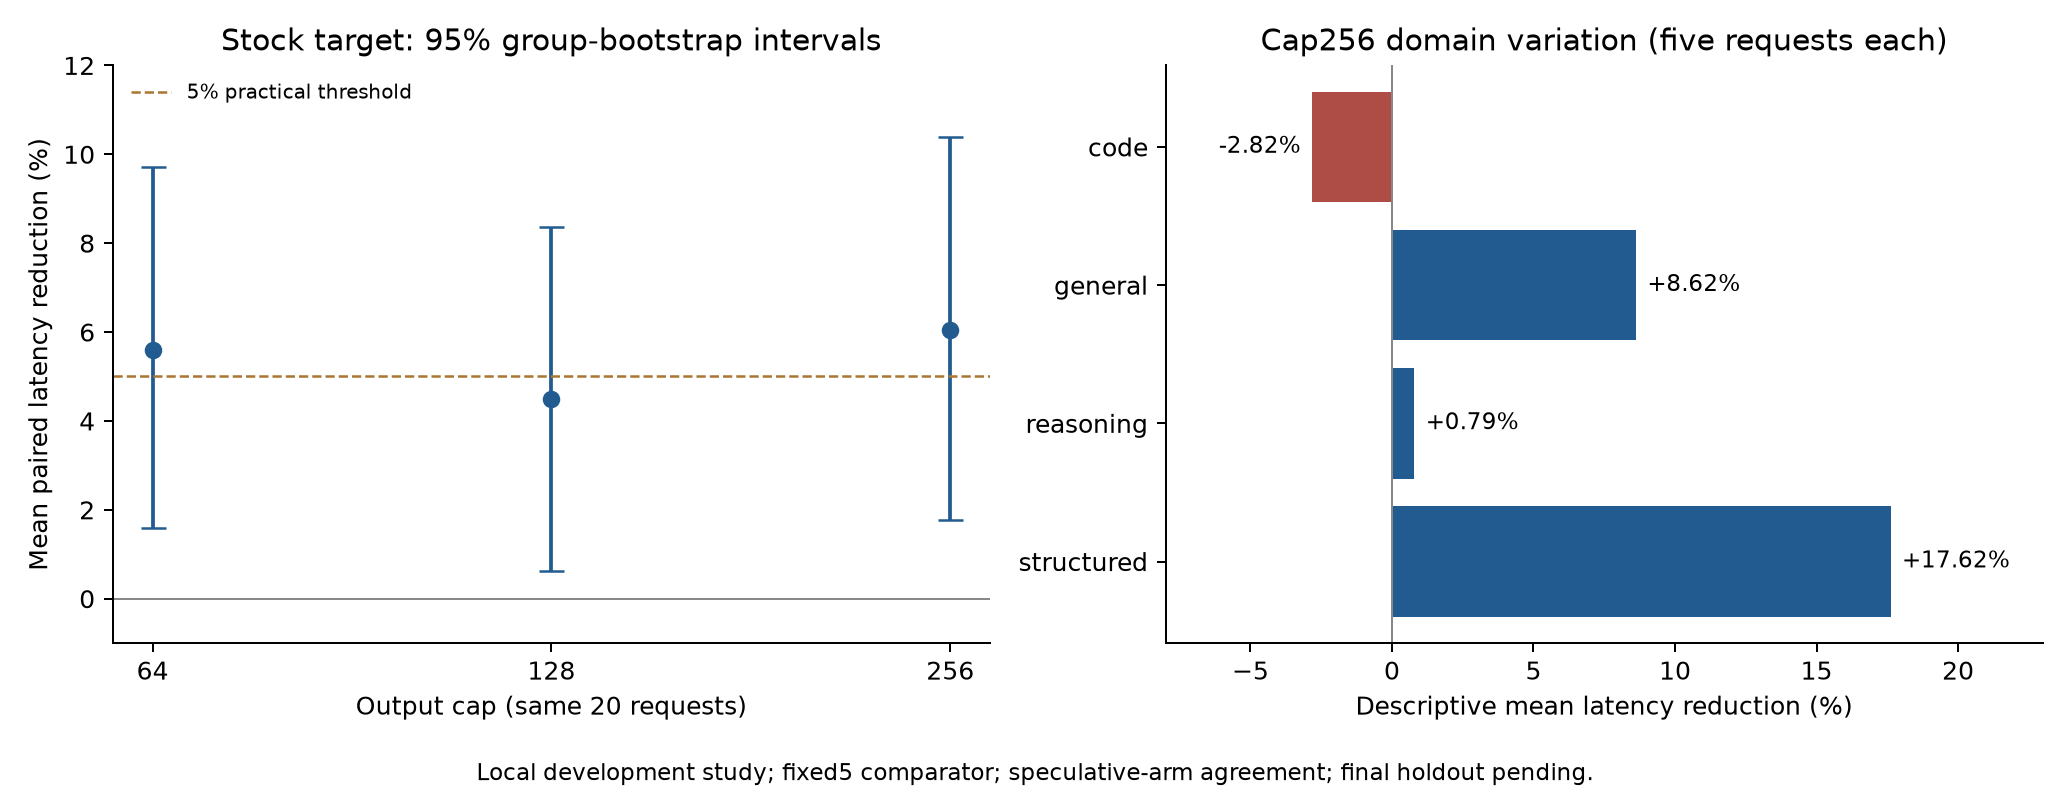
\includegraphics[keepaspectratio,alt={Stock-target cap results with group-bootstrap intervals and descriptive domain variation. The same twenty development requests are reused across caps.}]{figures/stock-results.png}}
\caption{Stock-target cap results with group-bootstrap intervals and
descriptive domain variation. The same twenty development requests are
reused across caps.}
\end{figure}

{\def\LTcaptype{none} % do not increment counter
\begin{longtable}[]{@{}
  >{\raggedright\arraybackslash}p{(\linewidth - 10\tabcolsep) * \real{0.1304}}
  >{\raggedleft\arraybackslash}p{(\linewidth - 10\tabcolsep) * \real{0.1739}}
  >{\raggedleft\arraybackslash}p{(\linewidth - 10\tabcolsep) * \real{0.1739}}
  >{\raggedleft\arraybackslash}p{(\linewidth - 10\tabcolsep) * \real{0.1739}}
  >{\raggedleft\arraybackslash}p{(\linewidth - 10\tabcolsep) * \real{0.1739}}
  >{\raggedleft\arraybackslash}p{(\linewidth - 10\tabcolsep) * \real{0.1739}}@{}}
\toprule\noalign{}
\begin{minipage}[b]{\linewidth}\raggedright
Output cap
\end{minipage} & \begin{minipage}[b]{\linewidth}\raggedleft
Requests
\end{minipage} & \begin{minipage}[b]{\linewidth}\raggedleft
Mean output tokens
\end{minipage} & \begin{minipage}[b]{\linewidth}\raggedleft
Paired latency reduction
\end{minipage} & \begin{minipage}[b]{\linewidth}\raggedleft
95\% interval
\end{minipage} & \begin{minipage}[b]{\linewidth}\raggedleft
Solo-divergent requests
\end{minipage} \\
\midrule\noalign{}
\endhead
\bottomrule\noalign{}
\endlastfoot
256 & 20 & 133.00 & 6.05\% & 1.77--10.38\% & 9/20 \\
128 & 20 & 97.35 & 4.48\% & 0.62--8.36\% & 7/20 \\
64 & 20 & 57.95 & 5.60\% & 1.59--9.70\% & 7/20 \\
\end{longtable}
}

\subsection{Primary result}\label{primary-result}

The cap-256 result meets all four recorded performance gates. Its
same-treatment null is −0.073\% with interval −0.844--0.708\%. The p95
request-mean latency change is −10.47\%, with interval −22.82 to
−1.66\%. The saved verdict nonetheless remains
\texttt{EXPLORATORY\_CANDIDATE\_FASTER}, \texttt{research\_only=true},
and \texttt{release\_ready=false} --- gate passage does not override
these statuses.

\subsection{Where the benefit comes from, and where it does
not}\label{where-the-benefit-comes-from-and-where-it-does-not}

Only 12 of 20 cap-256 requests improved. Domain means were code −2.82\%,
general +8.62\%, reasoning +0.79\%, and structured +17.62\%; with only
five requests per domain, these are descriptive differences, not
independently confirmed population effects. The relationship between
gain and generated length was weak in this sample (correlation 0.127).
Short-decision share correlated more strongly with gain (0.483), but
neither association identifies a causal mechanism.

Only two cap-256 requests reached the cap, and increasing a cap does not
necessarily lengthen an EOS-terminated response. The non-monotonic gain
curve, the reused prompts, and the fixed cap order together prevent us
from claiming that output length alone determines performance;
acceptance history and cost information matter as well as workload
length.

\subsection{Predictor consistency, not
calibration}\label{predictor-consistency-not-calibration}

Recorded stock predictions were 5.93\%, 6.31\%, and 6.43\% at caps 64,
128, and 256. Measured-minus-predicted errors were −0.328, −1.826, and
−0.378 percentage points, and each prediction falls within its measured
interval --- satisfying the registry's \texttt{CONSISTENT} rule. But the
intervals are wide and the settings are correlated (same requests, same
machine, same day), so this is weak evidence of calibration rather than
precise agreement. S0-derived expected lengths also exceeded observed S1
lengths. We do not interpret three consistent settings as three
independent successful workload replications.

\subsection{Stronger static baseline and complete session
record}\label{stronger-static-baseline-and-complete-session-record}

The four-arm follow-up completed on 27 September 2026. Full capture
validation and provenance checks pass; recomputation from raw rows
exactly matches all base report fields. The following contrasts use all
20 requests and six repeats per arm.

{\def\LTcaptype{none} % do not increment counter
\begin{longtable}[]{@{}lrr@{}}
\toprule\noalign{}
Candidate versus baseline & Mean latency reduction & 95\% interval \\
\midrule\noalign{}
\endhead
\bottomrule\noalign{}
\endlastfoot
Adaptive versus fixed5 & 4.50\% & 0.49--8.52\% \\
Fixed3 versus fixed5 & 0.96\% & -5.18--6.86\% \\
Adaptive versus fixed3 & 2.76\% & -0.70--6.26\% \\
Duplicate fixed5 versus fixed5 & -0.006\% & -0.211--0.168\% \\
\end{longtable}
}

Fixed3 is the development-selected global static setting by its point
estimate, but the uncertainty is substantial. The adaptive policy has a
positive interval against fixed5 and exceeds the duplicate-control
variation, yet misses the 5\% practical-gain threshold. Its p95
request-mean latency is 12.61\% lower than fixed5 (relative-increase
interval -19.78\% to -1.83\%). These are development request means, not
production tail measurements, and superiority over fixed3 is unresolved.

{\def\LTcaptype{none} % do not increment counter
\begin{longtable}[]{@{}
  >{\raggedright\arraybackslash}p{(\linewidth - 4\tabcolsep) * \real{0.2727}}
  >{\raggedleft\arraybackslash}p{(\linewidth - 4\tabcolsep) * \real{0.3636}}
  >{\raggedleft\arraybackslash}p{(\linewidth - 4\tabcolsep) * \real{0.3636}}@{}}
\toprule\noalign{}
\begin{minipage}[b]{\linewidth}\raggedright
Domain (five requests each)
\end{minipage} & \begin{minipage}[b]{\linewidth}\raggedleft
Adaptive versus fixed5
\end{minipage} & \begin{minipage}[b]{\linewidth}\raggedleft
Fixed3 versus fixed5
\end{minipage} \\
\midrule\noalign{}
\endhead
\bottomrule\noalign{}
\endlastfoot
Code & -1.97\% & -18.72\% \\
General & 7.42\% & 9.57\% \\
Reasoning & -2.31\% & -1.19\% \\
Structured & 14.88\% & 14.20\% \\
\end{longtable}
}

The adaptive policy avoids much of fixed3's observed code loss but does
not eliminate it. These exploratory domain means do not support
selecting a domain router or claiming specialized generalization from
five cases.

The earlier three-arm S1 estimate remains +6.05\% (1.77--10.38\%). The
completed five-arm resident session measured adaptive versus fixed5 at
+1.38\% (-2.68--5.18\%), fixed3 versus fixed5 at -4.81\%
(-11.40--1.46\%), and the local TapOut cap-4 adapter versus fixed5 at
-1.29\% (-5.06--1.95\%). The present +4.50\% follow-up is additional
evidence, not a replacement for that inconclusive session. The requests
are reused and schedules/operating conditions differ, so these sessions
neither form independent workload replications nor isolate the effect of
a loader or an extra arm. No rerun was selected on the sign of its
result.

The first four-arm attempt stopped during loading after warning memory
pressure persisted for more than 180 seconds; no scored observations
were collected. Its technical retry completed with unchanged policy and
pressure limits. Both attempts are retained. The completed resident
phase recorded zero system-wide swapout pages and 6,543 advisory
pageouts. Timings are not marked provisional under the registered
amendment, but this is not a zero-paging claim and model-specific
attribution is unavailable.

\subsection{Cost mechanism and the refresh
candidate}\label{cost-mechanism-and-the-refresh-candidate}

All 480 corresponding scored outputs and round counts agree with the
preceding five-arm session; all 120 adaptive decision traces also agree
after excluding timing fields. Thus the different relative timing gains
do not arise from changed token outputs or changed policy decisions in
these captures.

One code request accounts for almost all of the mean code regression. It
takes 8.643 seconds under adaptive versus 7.877 under fixed5, a 9.72\%
slowdown, with 47 versus 36 verification rounds. All 29 short decisions
accept both proposals. Measured decision callbacks total about 0.587
milliseconds, versus 766 milliseconds of extra request latency. Callback
optimization alone cannot explain most of that gap; no per-round
wall-time decomposition identifies the complete cause.

The frozen policy first chooses short after deep observations accepting
2/4 and 3/4 proposals. Even after a 4/4 probe at round 16, old
observations keep it short until the next scheduled probe at round 32.
Full short acceptance does not reveal the acceptance of ungenerated
proposals. We therefore propose obtaining new deep evidence, rather than
assuming those proposals would succeed: if the baseline chooses short,
the latest eligible deep observation accepted 4/4, and the two preceding
short rounds each accepted 2/2, request a deep refresh. All other
selector rules and costs stay frozen.

Replay of the actual selector finds the first changed decision on three
requests, consistently over six repeats: at rounds 19, 19 and 52, before
the original next deep probes at 32, 32 and 64. Candidate replay stops
at that first changed action; subsequent acceptance, fidelity and
latency require new generation. The candidate was selected from spent
data, with the risk of extra deep probes that do not repay their cost.
Its subsequently completed evaluation is reported below; the
first-divergence replay is not a counterfactual prediction of latency or
later acceptance.

\subsection{Completed refresh comparison and loading
revision}\label{completed-refresh-comparison-and-loading-revision}

The refresh comparison completed on 27 September 2026 with all 480
scored observations, 160 warmups, 60 speculative parity captures and 20
solo references. A saved-data audit on 28 September validates complete
ordering, token/stop agreement and controller traces, and reproduces all
four statistical contrasts exactly from the raw capture. The committed
480-row timing export reproduces the timing statistics without models or
private prompt contents.

{\def\LTcaptype{none} % do not increment counter
\begin{longtable}[]{@{}lrr@{}}
\toprule\noalign{}
Candidate versus baseline & Mean latency reduction & 95\% interval \\
\midrule\noalign{}
\endhead
\bottomrule\noalign{}
\endlastfoot
Refresh versus fixed5 & 7.13\% & 2.99--11.34\% \\
Original adaptive versus fixed5 & 7.03\% & 2.87--11.22\% \\
Refresh versus original adaptive & 0.113\% & -0.075--0.335\% \\
Duplicate fixed5 versus fixed5 & 0.006\% & -0.042--0.056\% \\
\end{longtable}
}

Refresh's p95 request-mean relative latency change versus fixed5 is
-14.37\% (interval -23.53\% to -2.62\%). Its incremental mean benefit
over the original rule is not established. The predeclared selection
rule requires a positive lower bound for that contrast as well as the
fixed5 gain, duplicate-control and p95 conditions. That condition fails,
so the original adaptive policy remains the candidate for fresh
confirmation. Fixed5 remains the operational fallback; neither candidate
is approved for deployment. Fixed3 was not an arm in this session, so it
adds no new evidence of superiority over fixed3.

An earlier refresh attempt collected 439 of 480 scored observations
before loss of AC power; its partial timings are retained and excluded
from complete-session inference. Three subsequent comparison attempts
stopped before reference or scored generation because warning memory
pressure exceeded the registered 180-second allowance. A separate
untimed diagnostic attributed about 13 GB of compressed memory to the
model process; its process samples showed no comparably large foreign
workload. This narrows the residency diagnosis without identifying every
kernel or operating-system cause.

The bounded loader previously performed an explicit GPU reduction on
only the first retained array in each batch. The amended implementation
reads every retained array on the GPU before stabilization. An untimed
diagnostic then reached the expected model identity and 30 seconds of
normal pressure, ending at 1.59 GiB compressor occupancy. Small-array
checks confirm read coverage and unchanged weight values. These
observations support the loading intervention operationally; they are
not a randomized causal estimate of its effect or a performance result.

The completed comparison records the loading revision and diagnostic
hashes in its provenance; models, policy, requests and pressure limits
remain unchanged, and all four arms share the revised loader. During the
resident phase, system-wide swapout delta is zero and advisory pageout
delta is 22,864. Timings are not marked provisional under the registered
amendment, but model-specific pageout attribution is unavailable. The
amendment still does not satisfy the original 17 GB admission protocol.
Cross-session gain differences cannot be assigned to refresh or loading
alone. Nine of 20 solo-reference disagreements persist. This is another
spent-data development session, not independent workload confirmation.

\subsection{Incomplete confirmation and post-identity loading
observation}\label{incomplete-confirmation-and-post-identity-loading-observation}

Three subsequent fresh-confirmation attempts remained incomplete. The
original attempt and recovery R2 stopped during resident-memory
stabilization before generation. Recovery R1 passed loading and the
three spent-input capacity captures, then stopped when the quiet-machine
supervisor detected an AI application: it retained seven solo records
(six completed and one interrupted) and 18 speculative parity records,
with no warmup or scored rows. All attempted bundles and interrupted
records are retained; none supplies a confirmation latency estimate.
R2's outcome-blind public sample was explicitly amended after a
structured-domain quota shortfall to retain 37 WildBench requests and
add three disjoint IFEval instruction prompts. That composite is not
exclusively natural user traffic, and IFEval's prior development use
prevents a dataset-level independence claim. These preparations did not
consume the protected original final holdout.

A separate untimed diagnostic on 28 September tested an additional
loading step after unchanged full runtime-identity construction and
verification: bounded GPU reductions read every retained target
parameter array (1,847 arrays in 57 batches) and drafter array (31
arrays in one batch), followed by the existing normal-pressure hold. It
completed with no token generation and zero recorded global swapout-page
increase. Global compressor occupancy was 6.644 GiB before the added
reads, 1.394 GiB immediately afterward and 1.353 GiB at the end of the
hold. The observation used the same model weights, runtime identity and
original memory-pressure limits; a separate 20 GiB disk-headroom
safeguard had been added after disk-full errors. The serving service
remained stopped with its recipe unchanged.

These observations support testing the loading change under inference,
not claiming that residency or request latency has been repaired. Global
wired memory rose briefly to 16.294 GiB but was 1.916 GiB at the end of
the hold. The process-level \texttt{top} CMPRS reading remained 9179M,
inconsistent with a straightforward current-live-memory interpretation
of the global compressor counts; that accounting discrepancy is
unresolved. The diagnostic includes measurement overhead and is not a
controlled causal comparison. A reduced evidence export and CPU-only
audit retain the batch coverage, stage values and source hashes without
prompt contents or process details. A separate generation-capacity and
speculative-parity check on an already-used request is required before
another newly registered fresh confirmation. No solo-equivalence, speed,
deployment or full-residency claim follows from this load-only pass.

\section{Fidelity: specifying the reference
computation}\label{fidelity-specifying-the-reference-computation}

\subsection{What the observed agreement
means}\label{what-the-observed-agreement-means}

The stock captures agree among the speculative arms in generated token
IDs and stopping outcomes, including the dedicated parity captures and
the recorded warmup/scored executions. We call this
\textbf{speculative-arm agreement}: it supports attributing the timing
difference between arms to policy, under the tested shared verifier. It
does \emph{not} establish equality with target-only decoding, equality
of sampled distributions, semantic correctness, or the absence of
cache-state defects.

At cap 256, 9 of 20 requests differed from the solo reference. We report
this directly; calling the result unqualified ``lossless decoding''
would conceal the reference against which the observations actually
hold.

\subsection{Numerical diagnostics and excluded speed
evidence}\label{numerical-diagnostics-and-excluded-speed-evidence}

Earlier modified-target probes localized a first divergence to
finite-precision behavior. One capture found a bf16 head tie at 27.375
versus 27.375, while an fp32 projection favored the other token by a
margin smaller than one bf16 unit at that magnitude. Additional
hidden/head comparisons implicated execution-regime differences rather
than simple disagreement between two head kernels on the same hidden
state. A one-sided near-tie certificate passed three diagnostic requests
and failed a fourth; subsequent analysis found the tie on the other arm,
and that failed certificate remains part of the record.

These earlier probes do not establish the numerical cause of the nine
stock-target divergences. The output-level inventory below classifies
their consequences; common-prefix cache-state checks, logit margins and
higher-precision controls are still required to distinguish
implementation defects from finite-precision effects. It would also be
wrong to claim bf16 makes exact agreement universally unattainable:
precision, kernels, model, and execution design all matter.

A serial-verification experiment achieved an apparent 10.13\% policy
gain while satisfying its solo reference, but it executed one target
forward per proposal rather than the served batched verifier. Because
block shortening then changes a different cost structure, we exclude
that number from the principal served-recipe latency table. It is useful
diagnostic evidence, not a stock replication of batched performance.

\subsection{Output-level classification of the nine stock
divergences}\label{output-level-classification-of-the-nine-stock-divergences}

A saved-token audit reconstructs the first differing token on all nine
cap256 requests. Five cases change open-ended content or continuations;
two multiple-choice cases retain the same selected answer while changing
explanations; one changes JSON structure; and one terminates in the solo
arm while the speculative arm continues. No divergent pair is
established as merely a harmless formatting change.

The JSON case is valid JSON on both paths but uses different keys and
nesting, so it is not schema-equivalent. The early-stop case ends at 28
tokens under solo and 53 under speculation; both ultimately record EOS,
showing why matching final stop labels alone is insufficient. The same
selected multiple-choice answer does not imply identical explanations or
a general semantic-equivalence guarantee. The narrative and rubric cases
contain substantive content differences. Shared instruction violations
also occur, so neither path can be treated as a task-quality oracle.

First divergence positions are 4, 13, 14, 27, 35, 37, 53, 142 and 220
(zero based). The captures do not contain matched-prefix logits,
recurrent/KV-state digests or higher-precision controls at these
positions. Their numerical cause remains unresolved. A follow-up must
compare both paths under the same forced prefix before attributing a
mismatch to rollback or precision, and must keep any altered-verifier
timings separate from the policy benchmark.

\section{Supporting personalization and implementation
evidence}\label{supporting-personalization-and-implementation-evidence}

\subsection{Four-week personalization: a scoped negative
result}\label{four-week-personalization-a-scoped-negative-result}

The original registration required personal-holdout acceptance to
improve by ten absolute percentage points. Day 0 recorded 57.63\%,
giving a threshold of 67.63\%. The Day-28 frozen curve completed 20 of
20 requests with mean 56.935\% --- 10.695 percentage points below that
threshold. No drafter was promoted. This is a failure of the registered
experiment, not proof that every personalization design is ineffective.

Training variants included A0, A1, B, Bp, and P. The archived
matched-control analysis reports P minus stock at approximately −2.159
percentage points and P minus its matched A0 control at +0.195, with an
interval spanning zero. Decreasing training loss did not translate into
improved acceptance. The stock-target headroom test in Section 8.4 has
since completed: its acceptance-targeted arm measured a sub-bar,
non-significant +1.4 pp and its distillation arm +0.2 pp, with outputs
byte-identical throughout.

The training investigation also surfaced practical objective/runtime
mismatches. Small norm updates could be lost when training or export
rounded them into bf16. The drafter consumes post-final-normalization
hidden state, so supervising a different tensor changes the learning
problem. One label interpretation was later retracted after checking the
pinned speculative path: repetition processors used by ordinary
generation did not enter that verifier, so raw-argmax and
penalized-chain labels were not interchangeable. These are
implementation findings from the recorded source and diagnostics, not
proof that repairing them guarantees a positive training transfer.

The four-criterion claim also had reporting and cadence gaps: weekly
measurements were absent at several scheduled points. The Day-28 weekly
stock-drafter suite on a different mlp3 target completed 24 prompts at
55.741667\%, above its own 48.55\% floor, but this cannot repair the
missing weeks or replace the curve target. The 169-prompt candidate
referee was not run, and a historical canary-error refusal lacks both
referee numbers. Finally, a Day-28 validator accepted service snapshots
with unsupported smoke/review assertions --- its schema status is not
proof those assertions occurred. These qualifications accompany, rather
than soften, the negative closure.

\subsection{Correct profiling must reproduce the serving
path}\label{correct-profiling-must-reproduce-the-serving-path}

A corrected verification microbenchmark measured 154.696 ms for the
served forward versus 144.011 ms for a plain forward, with ten repeats
in the selected stable run. The discrepancy previously described as
barrier overhead in fact came from different execution paths, including
state capture and head evaluation, and the old explanation has been
withdrawn. This illustrates why numerically similar timing cells are not
interchangeable without checking entry-point equivalence first.

Drafter decomposition identified repeated shared output-head reads as a
substantial cost in its tested setting. Those phase timings constrain
specific optimization hypotheses, but synchronized microbenchmarks,
single prefixes, and constructed totals are not end-to-end speed
measurements. The completed same-verifier static comparison in Section
6.4 now measures this question directly; its uncertainty still prevents
a claim that adaptation outperforms the best fixed setting.

\subsection{Prefix state and persistent
memory}\label{prefix-state-and-persistent-memory}

An exact-prefix resident study completed 45 rebuild/reuse pairs over
three development requests, with matching within-regime output IDs and
stop reasons. Entry state included KV, recurrent GDN and position state,
and complete hidden history. Cross-regime exact-versus-MTP output
differences persisted. Because the study primed entries separately and
lacked an operational reuse trace, it cannot establish workload-wide
cache ROI. Persistent computational memory and approximation proposals
must retain this distinction: a valid state-restoration check is not a
production amortization result, nor is it evidence of trained
approximation quality.

\subsection{A pre-registered stock-target headroom test:
INCONCLUSIVE}\label{a-pre-registered-stock-target-headroom-test-inconclusive}

After the four-week closure, a separate pre-registered test asks whether
self-distillation on the owner's own traffic gives the stock target's
drafter headroom that the generic head lacks. Its decision rule was
fixed before any data: on a held-out EVAL set of 92 owner prompts,
greedy, cap 256, block 5, a trained 4-bit drafter must improve
acceptance over the 4-bit generic head by at least 3.0 percentage
points, with the lower bound of a Bonferroni 97.5 \% bootstrap interval
(10,000 resamples, seed 0) above zero; if both arms' upper bounds fall
below 3.0 points the verdict is CAPPED, and otherwise INCONCLUSIVE, with
one replication on fresh EVAL prompts and no pooling. Two objectives are
registered, knowledge distillation and a total-variation/KL hybrid
expected to be the weaker, each selected on a separate 32-prompt DEV set
by served acceptance, never by an offline proxy. Prompts are split by a
fixed-prefix SHA-256 of their normalised text with a character 5-gram
leakage filter (162 TRAIN prompts after filtering).

The first capture smoke found a defect in the registration rather than
the code. Continuations ran to 1,024 tokens while the teacher-forced
label forward accepts at most 512 tokens of prompt plus response, so 23
of 24 generations were discarded and the survivors were selected on
response length (457 of 18,683 tokens labelled). An addendum, written
before any corpus row existed and authorised by the owner, caps each
continuation at the label room, min(1,024, 512 − prompt length). Because
the target is causal, the kept tokens and their labels are exactly those
the uncapped run would have produced; the cost is that no training
context exceeds 512 tokens, and 6 of the 92 EVAL prompts are longer than
that. The change was made after a smoke had been seen; the smoke exposed
row lengths and statuses only, and no drafter or acceptance figure
existed.

Capture A, over the original 162 TRAIN prompts, ran in two sessions
(10.7 and 5.7 hours) and crossed its floor after nine full passes:
411,866 labelled tokens in 1,563 rows, with 17 duplicates, 40 rows
refused before generation for the four prompts already over the ceiling,
and none discarded after generation. The pass count fell inside the
registered expectation of six to ten; the 16.4 capture hours fell below
the registered 20 to 35.

Before any training, three further addenda widened the training
population with more of the owner's own prompts under the same rules:
prompts mirrored after the split, user-typed messages from local
coding-assistant transcripts and sessions, and eleven months of the
owner's prompt history. Only prompts whose registered split bucket is
TRAIN were eligible; the rest were discarded rather than moved into DEV
or EVAL, and any prompt with character 5-gram Jaccard similarity of at
least 0.80 to a DEV or EVAL prompt was removed. Of 9,455 eligible
prompts, a fixed-size sample of 2,000 was drawn by a salted hash of the
text, and the corpus floor rose to 800,000 tokens. DEV, EVAL, the bar
and the interval did not change. Train and test sources are therefore
unequal --- EVAL remains mirrored traffic from late September --- and
this is reported next to the verdict.

The second capture, over those 2,000 prompts, exposed a defect in a
guard rather than in the registration. Both the capture driver and the
referee refused any rendered prompt containing a substring that marks a
mis-rendered message list; one owner prompt quoted that substring, and
the capture stopped after 47 rows. The guard was narrowed to refuse only
occurrences that the template added beyond the message's own text,
verified on the two affected prompts (one TRAIN, one DEV), and the
capture restarted from scratch under the corrected driver after its own
smoke run. The interrupted rows are retained as evidence and excluded
from the corpus. A further addendum then fixed the training recipe, the
step-count probe, the validity gate and the DEV selection statistic
before any training, after a code review found that the trainer's
defaults would otherwise keep the best snapshot by an offline proxy and
stop early on it, which the registration forbids.

\textbf{Length selection in the training distribution (disclosed from an
audit on 2 October 2026, before any DEV or EVAL decoding of a trained
drafter; Addendum 6).} The corpus is not a sample of the target's
unconstrained behaviour, and the following limitations are stated
plainly. (i) The generation cap makes a large share of rows end
mid-response. Capture A: 510 of 1,563 rows (33 \%) hit the cap, carrying
51 \% of its labelled tokens. Capture B: 916 of 1,934 rows (47 \%),
carrying 66 \% of its tokens. Over the combined corpus actually trained
on: 1,426 of 3,497 rows (41 \%), carrying 60 \% of its 1,067,434 tokens.
The share rises with prompt length in both captures (capture A, by band:
29.1 \% of rows for prompts under 64 tokens, 48.0 \%, 15.8 \%, 66.7 \%,
then 100 \% for prompts of 384 to 511; capture B: 45.6 \%, 69.8 \%, 57.9
\%, 90.9 \%, 88.9 \%). Capped rows carry no end-of-sequence label. The
audit recorded as unverified whether a response ending exactly at its
cap is flagged as capped; it is, and necessarily so, because the flag
tests \texttt{n\_tokens\ \textgreater{}=\ generation\_cap} and
generation stops at the cap, so every flagged row sits exactly at it.
The flag therefore cannot separate a truncated response from one that
happened to end on its last permitted token, and these shares are upper
bounds on genuine truncation. (ii) Prompts of 512 tokens or more have no
label room and are refused before generation (40 refusals across capture
A's nine passes, from 4 of its 162 prompts; 58 of capture B's 2,000
prompts); a prompt over the 16,000-token budget is also dropped (8 in
capture B, none in A). The corpus therefore contains no long-context
example, while 6 of 92 EVAL prompts and 2 of 32 DEV prompts are 512
tokens or longer, and 11 of 92 EVAL prompts, including those 6, can
decode past position 512 under the 256-token EVAL cap (prompt length of
257 or more) (at most about 8.7 \% of EVAL decode positions); the
addendum that named the exclusion counted only the six. EVAL and DEV
have no 512-token ceiling. (iii) The trainer never draws a window from a
row shorter than 68 tokens (window 64 plus K 3 plus 1); this is not
logged, and 113 of the corpus's 3,497 rows are unusable for that reason
(88 from capture A, 25 from capture B). It had been noted only in the
project's working notes. (iv) Prompt-history rows containing pasted
content (1,846) were excluded from the extension, which removes some of
the longest prompts. All figures in this paragraph are final: both
captures are complete, and they are re-derived by
\texttt{analysis/headroom\_length\_audit\_final.py} from the capture
manifests and the corpus manifest. That script reproduces every
capture-A figure the 2 October audit registered, which is the check that
the final capture-B values were computed the same way. These are
limitations of the training distribution and are reported beside every
result; they do not alter the bar, the interval or the EVAL set.

\textbf{Training and selection.} Both arms trained for the registered
22,776 steps (knowledge distillation completing 13 October, the
acceptance objective 15 October 2026), with the whole 424.7 M-parameter
head trainable except seven normalisation vectors frozen against bf16
rounding. The validity gate passed for both, and the step-0 4-bit
snapshot reproduced the served drafter \texttt{orca-mtp-q4} by tensor
checksum, so the comparator is the served drafter itself. DEV selection,
by served acceptance on the 32 DEV prompts and never by the offline
proxy, chose step 2,847 for \textbf{both} arms: the first snapshot after
step 0, about 12 \% of the budget. Against step 0's 49.19 \%, knowledge
distillation's eight trained snapshots spanned 48.54--50.15 \% with no
trend; the acceptance objective's eight all exceeded step 0
(50.02--51.46 \%), the first the highest and the rest flat within about
one point. Whatever the acceptance objective learns is present by step
2,847, at a learning rate still at its \(3 \times 10^{-6}\) peak; the
following 20,000 steps added nothing the DEV instrument could see.

\textbf{Verdict: INCONCLUSIVE} (EVAL run 15 October 2026, 16:38--18:21
AEDT, one quiet session, 92 prompts × 3 arms, pair rate 1.0, no
truncation, no voided rows). On the registered metric --- per-prompt
acceptance, accepted over drafted tokens, paired against the comparator
with a 97.5 \% Bonferroni bootstrap interval --- knowledge distillation
measured \textbf{+0.18 pp} {[}−1.42, +2.14{]} and the acceptance
objective \textbf{+1.44 pp} {[}−0.83, +4.13{]}. Neither clears +3.0 pp
with a lower bound above zero (HEADROOM); neither has an upper bound
below +3.0 pp (CAPPED). Output text was byte-identical across all three
arms on all 92 prompts, and generated length was identical on all 92, so
the lossless-by-verification property held throughout.

\textbf{Secondaries, descriptive only.} The registered per-position
ladder, pooled over rounds at block 5, was {[}0.800, 0.596, 0.420,
0.293{]} for the comparator, {[}0.809, 0.589, 0.408, 0.279{]} for
knowledge distillation and {[}0.810, 0.594, 0.413, 0.289{]} for the
acceptance objective: about one point gained at the first draft position
and nothing, or slightly less, at positions two to four. This is the
opposite of the shape the trainer's offline chain proxy reported for the
same checkpoints, where gains grew with depth (+1.6, +2.4 and +5.6
points at positions one to three); Amendment 37's prohibition on
selecting by that proxy was vindicated on its first new objective
family. Pooled over all drafted tokens rather than averaged per prompt
--- the aggregation that governs wall-clock speed --- the acceptance
objective's acceptance is 52.73 \% against the comparator's 52.80 \%, a
difference of −0.07 pp, and generation speed is unchanged (median 13.32
against 13.38 tokens/s; paired median −0.24 \%). The per-prompt average
and the pooled rate disagree because the per-prompt gain, where it
exists, sits in requests that drafted few tokens: a post-hoc split at
the median number of rounds, which depends on the decode and is
therefore outside the registered subsets, gives +3.15 pp {[}−1.15,
+7.45{]} on the shorter half and −0.26 pp {[}−1.02, +0.49{]} on the
longer half, a 3.4-point difference at z = 1.5. The registered Addendum
6 subsets, fixed from prompt length alone: S\_rest (81 prompts) +1.62 pp
{[}−0.50, +4.25{]} for the acceptance objective and −0.07 pp {[}−1.44,
+1.47{]} for knowledge distillation; S\_crossing-only (5 prompts of
257--511 tokens, whose decode passes the corpus's 512-token ceiling)
−2.97 pp {[}−4.95, −1.34{]} and −2.76 pp {[}−4.74, −1.03{]};
S\_refused-in-TRAIN (6 prompts of 512 tokens or more) +2.78 pp
{[}−13.25, +24.64{]} and +5.95 pp {[}−4.43, +24.41{]}. No subset result
is promoted; the five-prompt interval is noted because its sign is
consistent with the length limitation the addendum disclosed, not as
evidence of it.

\textbf{Power, and the replication.} The per-prompt paired spread on
EVAL was 10.8 pp for the acceptance objective and 7.7 pp for knowledge
distillation. The design was adequately powered for its bar: at this
spread a true +3.0 pp effect clears a lower bound of zero with about 65
prompts. The effect measured is smaller than the bar, and the registered
replication on the next 40 EVAL-eligible prompts would have a half-width
near 3.8 pp, which can return neither HEADROOM nor CAPPED for any point
estimate near the one observed; about 280 prompts would be needed to
place the lower bound above zero at +1.4 pp, or the upper bound below
+3.0 pp.~That replication has not been run, and the registration does
not permit pooling it with this result.

\textbf{Reading.} Taken with Section 8.1, the result is a dissociation,
now measured on the served path rather than inferred offline:
cross-entropy distillation lowered held-out loss by 26 \% and moved
acceptance by +0.2 pp; an acceptance-targeted objective left loss high
and moved the per-prompt average by +1.4 pp, concentrated at the first
draft position and in short requests, with no change in pooled
acceptance or generation speed. It is a small, sub-bar effect whose
interval does not exclude zero. Whether it reflects the owner's traffic
or adaptation of a third-party head to the stock target is not tested
here; the generic control the registration reserves for a HEADROOM
verdict was not triggered.

\section{Cross-machine reproducibility of the
analysis}\label{cross-machine-reproducibility-of-the-analysis}

A separate Apple M4 MacBook Air (Mac16,12, 10 CPU cores, 16 GB unified
memory) reran the analysis on 27 September 2026 using the exported
four-arm timing data. The returned environment records macOS 26.6.2,
Python 3.12.14, NumPy 2.5.2 and pytest 9.1.1. NumPy and pytest match the
audit pins; Python differs by one patch version from the original
3.12.13 environment. No model loading, inference or training was part of
this audit.

The unchanged reproduction script checked complete coverage of all 480
scored rows (20 requests, four arms and six repeats), recomputed
per-request means and exactly matched all fields of the four saved
bootstrap comparison dictionaries. This includes gain and p95 estimates,
confidence intervals, resample counts and seed. The reproduced mean
gains were 4.504\% for adaptive versus fixed5, 0.961\% for fixed3 versus
fixed5, 2.756\% for adaptive versus fixed3, and -0.006\% for the
duplicate fixed5 control, with the intervals in Section 6.4 unchanged.
Recomputing these results does not add observations or narrow their
uncertainty: the 5\% mean-gain gate still fails, and adaptive
superiority over fixed3 remains unestablished.

The selected CPU report/status suite completed with 44 passed, 13
skipped and zero failed tests. All skips were existing conditions for
the unavailable sibling Whetstone repository; no assertions or skip
conditions were changed. A supplemental arithmetic check matched the
four domain pairs and timing gates. The return verification checked 40
evidence-manifest entries and the archive checksum, and matched all 12
original exported files against the first Mac's hashes. This establishes
consistency with the supplied export; the second Mac did not
independently authenticate the commit against GitHub.

This is cross-machine reproducibility of saved-data analysis and
selected CPU tooling, not replication of model outputs, runtime fidelity
or inference latency. A separately prepared 4B M4 benchmark was present
in the returned directory, but no attempt records or timing results were
found in that copy. Its execution remains unverified and supplies no
performance evidence. The original 27B inference measurements therefore
remain a single-machine study.

\section{Limitations and next
evidence}\label{limitations-and-next-evidence}

The principal inference study has one machine, one target/drafter pair,
20 stock development requests, a restricted greedy recipe, and limited
environmental monitoring. The original final partition remains prepared
but unexecuted in the inspected registration; a failed or inconclusive
final result would still be reported in the manuscript. Missing
selection-chain evidence for the reported tuned stage-2 experiment must
be recovered --- its archived +7.74\% headline is not used as an
independently audited result here. The stock-target headroom test in
Section 8.4 completed on 15 October 2026 with the registered verdict
INCONCLUSIVE: +1.4 pp {[}−0.8, +4.1{]} for the acceptance objective and
+0.2 pp {[}−1.4, +2.1{]} for distillation on 92 prompts, neither
clearing the +3.0 pp bar nor ruling it out, and no change in pooled
acceptance or generation speed. Its registered 40-prompt replication is
underpowered to resolve it at the observed spread; a larger fresh-prompt
replication declared before it is run, or a stronger arm, are the open
next steps.

The same-verifier static baseline, local TapOut-adapter and refresh
comparisons are now complete, but remain small, spent-data experiments.
The predeclared selection rule retains the original policy. The next
performance question is whether it survives fresh requests against both
fixed3 and fixed5. The separate 40-request confirmation design uses ten
groups per code/general/reasoning/structured domain, split before
generation into two balanced sessions. Its public-sample recovery
amendments and three incomplete attempts are described in the
incomplete-confirmation subsection above; no completed
fresh-confirmation estimate is available. The R2 composite comprised 37
WildBench requests and three IFEval prompts, with documented input/ID
exclusions and remaining historical source-mapping limits. A future
confirmation must follow successful spent-input capacity/parity
validation, preserve the failed attempts, exclude previously reserved
requests under its declared rules, and seal its population, loading
amendment and analysis before outcomes are observed. It does not amend
or consume the protected original final partition. A per-request best-K
oracle is only a descriptive bound. A broader numerical-fidelity audit,
actual public or consented private workload replay, and timed inference
on a second hardware tier remain necessary. The M4 audit above
reproduces the analysis only. Another run on this Mac would test
within-machine repeatability, not hardware generality. Public-traffic
and owner-traffic forecasts presently lack corresponding timed
validation.

Reproducibility also requires an exact measurement-time environment,
upstream model identity, capture provenance, and a reviewed public
artifact package. Private prompts, mirrored owner traffic, holdout
contents, machine-process records, and credentials must not be included
automatically. Source licensing and dataset redistribution must be
resolved before release, and no power measurement supports an energy
claim.

\section{Application integration and
conclusion}\label{application-integration-and-conclusion}

The intended integration boundary is a provenance-bearing inference
event: run, request, model, fixture, policy, timing, acceptance, and
refusal identities. Such events are what any downstream orchestration,
training or analytics consumer would need in order to attribute observed
behaviour to a specific model and policy, and the schema is deliberately
specified independently of any particular consumer. Evaluation reference
labels and final-holdout records remain outside online training. These
are proposed connections, not measured deployed integrations.

The completed development sessions support average latency benefits
relative to fixed block 5 under their tested verifier, while superiority
over fixed block 3 remains uncertain. The refresh follow-up does not
establish an incremental benefit over the original rule, so the
predeclared selection rule retains that original candidate. The explicit
GPU residency loading revision enables a completed session after
repeated pressure refusals, without establishing its isolated effect on
measured gains. Extra verification rounds provide a concrete
code-regression hypothesis, and output-level divergence classification
narrows the fidelity claim without resolving its numerical cause. The
failed personalization window and the corrected profiling claims explain
why adaptation, measurement, and promotion each need their own evidence.
The separate M4 audit establishes reproducibility of the saved-data
analysis, while cross-machine inference performance remains unmeasured
in the available record. The result is a foundation for further
confirmation, not authorization to enable adaptive speculation
generally.

\section{Appendix A. Typed decisions and
Nimble}\label{appendix-a.-typed-decisions-and-nimble}

An independent audit of 420 examples from 21 selected BANKING77 intents
reproduced 351 correct MLX decisions and 332 correct Nimble decisions,
with 369 matching predictions and a paired correctness discordance of 29
versus 10. This is an exploratory comparison of different models and
rendering paths, not a causal estimate of MTP's effect, and the
different loading and timing boundaries preclude a speed ratio. The case
study illustrates an application-quality endpoint; it is secondary to
the same-target policy experiment.

\section{Appendix B. Bonsai}\label{appendix-b.-bonsai}

Saved single-operation Bonsai checks support limited numerical claims,
not full-model qualification. The latest eight-prompt diagnostic
completed the first Bonsai arm with zero recorded nonfinite values, but
the Qwen arm never loaded and the repeat Bonsai arm was skipped ---
leaving zero paired prompts and no valid comparative-speed conclusion.
Human coherence review and a complete controlled comparison remain
pending. Missing arms must not be represented as zero-performance
baselines.

\bibliography{references.bib}

\end{document}
